% Options for packages loaded elsewhere
\PassOptionsToPackage{unicode}{hyperref}
\PassOptionsToPackage{hyphens}{url}
%
\documentclass[
]{article}
\title{Power Analysis for CSI online typing with patients with aphasia -
Summary}
\author{Kirsten Stark}
\date{08 Dezember, 2021}

\usepackage{amsmath,amssymb}
\usepackage{lmodern}
\usepackage{iftex}
\ifPDFTeX
  \usepackage[T1]{fontenc}
  \usepackage[utf8]{inputenc}
  \usepackage{textcomp} % provide euro and other symbols
\else % if luatex or xetex
  \usepackage{unicode-math}
  \defaultfontfeatures{Scale=MatchLowercase}
  \defaultfontfeatures[\rmfamily]{Ligatures=TeX,Scale=1}
\fi
% Use upquote if available, for straight quotes in verbatim environments
\IfFileExists{upquote.sty}{\usepackage{upquote}}{}
\IfFileExists{microtype.sty}{% use microtype if available
  \usepackage[]{microtype}
  \UseMicrotypeSet[protrusion]{basicmath} % disable protrusion for tt fonts
}{}
\makeatletter
\@ifundefined{KOMAClassName}{% if non-KOMA class
  \IfFileExists{parskip.sty}{%
    \usepackage{parskip}
  }{% else
    \setlength{\parindent}{0pt}
    \setlength{\parskip}{6pt plus 2pt minus 1pt}}
}{% if KOMA class
  \KOMAoptions{parskip=half}}
\makeatother
\usepackage{xcolor}
\IfFileExists{xurl.sty}{\usepackage{xurl}}{} % add URL line breaks if available
\IfFileExists{bookmark.sty}{\usepackage{bookmark}}{\usepackage{hyperref}}
\hypersetup{
  pdftitle={Power Analysis for CSI online typing with patients with aphasia - Summary},
  pdfauthor={Kirsten Stark},
  hidelinks,
  pdfcreator={LaTeX via pandoc}}
\urlstyle{same} % disable monospaced font for URLs
\usepackage[margin=1in]{geometry}
\usepackage{color}
\usepackage{fancyvrb}
\newcommand{\VerbBar}{|}
\newcommand{\VERB}{\Verb[commandchars=\\\{\}]}
\DefineVerbatimEnvironment{Highlighting}{Verbatim}{commandchars=\\\{\}}
% Add ',fontsize=\small' for more characters per line
\usepackage{framed}
\definecolor{shadecolor}{RGB}{248,248,248}
\newenvironment{Shaded}{\begin{snugshade}}{\end{snugshade}}
\newcommand{\AlertTok}[1]{\textcolor[rgb]{0.94,0.16,0.16}{#1}}
\newcommand{\AnnotationTok}[1]{\textcolor[rgb]{0.56,0.35,0.01}{\textbf{\textit{#1}}}}
\newcommand{\AttributeTok}[1]{\textcolor[rgb]{0.77,0.63,0.00}{#1}}
\newcommand{\BaseNTok}[1]{\textcolor[rgb]{0.00,0.00,0.81}{#1}}
\newcommand{\BuiltInTok}[1]{#1}
\newcommand{\CharTok}[1]{\textcolor[rgb]{0.31,0.60,0.02}{#1}}
\newcommand{\CommentTok}[1]{\textcolor[rgb]{0.56,0.35,0.01}{\textit{#1}}}
\newcommand{\CommentVarTok}[1]{\textcolor[rgb]{0.56,0.35,0.01}{\textbf{\textit{#1}}}}
\newcommand{\ConstantTok}[1]{\textcolor[rgb]{0.00,0.00,0.00}{#1}}
\newcommand{\ControlFlowTok}[1]{\textcolor[rgb]{0.13,0.29,0.53}{\textbf{#1}}}
\newcommand{\DataTypeTok}[1]{\textcolor[rgb]{0.13,0.29,0.53}{#1}}
\newcommand{\DecValTok}[1]{\textcolor[rgb]{0.00,0.00,0.81}{#1}}
\newcommand{\DocumentationTok}[1]{\textcolor[rgb]{0.56,0.35,0.01}{\textbf{\textit{#1}}}}
\newcommand{\ErrorTok}[1]{\textcolor[rgb]{0.64,0.00,0.00}{\textbf{#1}}}
\newcommand{\ExtensionTok}[1]{#1}
\newcommand{\FloatTok}[1]{\textcolor[rgb]{0.00,0.00,0.81}{#1}}
\newcommand{\FunctionTok}[1]{\textcolor[rgb]{0.00,0.00,0.00}{#1}}
\newcommand{\ImportTok}[1]{#1}
\newcommand{\InformationTok}[1]{\textcolor[rgb]{0.56,0.35,0.01}{\textbf{\textit{#1}}}}
\newcommand{\KeywordTok}[1]{\textcolor[rgb]{0.13,0.29,0.53}{\textbf{#1}}}
\newcommand{\NormalTok}[1]{#1}
\newcommand{\OperatorTok}[1]{\textcolor[rgb]{0.81,0.36,0.00}{\textbf{#1}}}
\newcommand{\OtherTok}[1]{\textcolor[rgb]{0.56,0.35,0.01}{#1}}
\newcommand{\PreprocessorTok}[1]{\textcolor[rgb]{0.56,0.35,0.01}{\textit{#1}}}
\newcommand{\RegionMarkerTok}[1]{#1}
\newcommand{\SpecialCharTok}[1]{\textcolor[rgb]{0.00,0.00,0.00}{#1}}
\newcommand{\SpecialStringTok}[1]{\textcolor[rgb]{0.31,0.60,0.02}{#1}}
\newcommand{\StringTok}[1]{\textcolor[rgb]{0.31,0.60,0.02}{#1}}
\newcommand{\VariableTok}[1]{\textcolor[rgb]{0.00,0.00,0.00}{#1}}
\newcommand{\VerbatimStringTok}[1]{\textcolor[rgb]{0.31,0.60,0.02}{#1}}
\newcommand{\WarningTok}[1]{\textcolor[rgb]{0.56,0.35,0.01}{\textbf{\textit{#1}}}}
\usepackage{graphicx}
\makeatletter
\def\maxwidth{\ifdim\Gin@nat@width>\linewidth\linewidth\else\Gin@nat@width\fi}
\def\maxheight{\ifdim\Gin@nat@height>\textheight\textheight\else\Gin@nat@height\fi}
\makeatother
% Scale images if necessary, so that they will not overflow the page
% margins by default, and it is still possible to overwrite the defaults
% using explicit options in \includegraphics[width, height, ...]{}
\setkeys{Gin}{width=\maxwidth,height=\maxheight,keepaspectratio}
% Set default figure placement to htbp
\makeatletter
\def\fps@figure{htbp}
\makeatother
\setlength{\emergencystretch}{3em} % prevent overfull lines
\providecommand{\tightlist}{%
  \setlength{\itemsep}{0pt}\setlength{\parskip}{0pt}}
\setcounter{secnumdepth}{-\maxdimen} % remove section numbering
\ifLuaTeX
  \usepackage{selnolig}  % disable illegal ligatures
\fi

\begin{document}
\maketitle

\hypertarget{load-packages}{%
\section{load packages}\label{load-packages}}

\begin{Shaded}
\begin{Highlighting}[]
\FunctionTok{library}\NormalTok{(tidyr)}
\FunctionTok{library}\NormalTok{(dplyr)}
\FunctionTok{library}\NormalTok{(devtools)}
\FunctionTok{library}\NormalTok{(MASS)}
\FunctionTok{library}\NormalTok{(lme4)}
\FunctionTok{library}\NormalTok{(lmerTest)}
\FunctionTok{library}\NormalTok{(simr)}
\FunctionTok{library}\NormalTok{(pbkrtest)}
\FunctionTok{library}\NormalTok{(testthat)}
\FunctionTok{library}\NormalTok{(ggplot2)}

\FunctionTok{rm}\NormalTok{(}\AttributeTok{list =} \FunctionTok{ls}\NormalTok{())}

\NormalTok{today }\OtherTok{\textless{}{-}} \FunctionTok{Sys.Date}\NormalTok{()}
\NormalTok{today }\OtherTok{\textless{}{-}} \FunctionTok{format}\NormalTok{(today, }\AttributeTok{format=}\StringTok{"\%d\%m\%y"}\NormalTok{)}

\CommentTok{\# Set number of iterations }
\NormalTok{n\_iter }\OtherTok{=} \DecValTok{1000}
\FunctionTok{set.seed}\NormalTok{(}\DecValTok{99}\NormalTok{)}
\end{Highlighting}
\end{Shaded}

\hypertarget{load-data-from-lorenz-doering-van-scherpenberg-pino-abdel-rahman-obrig-2021}{%
\section{Load data from Lorenz, Doering, van Scherpenberg, Pino, Abdel
Rahman, \& Obrig
(2021)}\label{load-data-from-lorenz-doering-van-scherpenberg-pino-abdel-rahman-obrig-2021}}

In this lab-based study, people with Aphasia did a CSI task with 3
repetitions in two subsequent weeks. Both testing sessions had different
items. Additionally, participants also did a CSI task with compounds
(not relevant here).\\
The data loaded here are already cleaned for errors and participants.

\begin{Shaded}
\begin{Highlighting}[]
\CommentTok{\# load data}
\NormalTok{df }\OtherTok{\textless{}{-}} \FunctionTok{read.csv2}\NormalTok{(here}\SpecialCharTok{::}\FunctionTok{here}\NormalTok{(}\StringTok{"data"}\NormalTok{, }\StringTok{"power{-}analysis"}\NormalTok{,}
                \StringTok{"Doeringetal\_PWA\_naming\_simple\_nouns\_data\_for\_modelling.csv"}\NormalTok{))}

\CommentTok{\# subset the relevant columns}
\NormalTok{df }\OtherTok{\textless{}{-}}\NormalTok{ df }\SpecialCharTok{\%\textgreater{}\%} 
  \FunctionTok{filter}\NormalTok{(error}\SpecialCharTok{==}\DecValTok{1}\NormalTok{) }\SpecialCharTok{\%\textgreater{}\%} 
    \CommentTok{\# repet\_trig = repetition (151,152,153 is 1,2,3), }
    \CommentTok{\# wh = testing session 1 and 2, }
    \CommentTok{\# cat\_nr = 18 categories (à 5 members each)}
\NormalTok{  dplyr}\SpecialCharTok{::}\FunctionTok{select}\NormalTok{(}\FunctionTok{c}\NormalTok{(subject, Ordinal\_position, RT, }
\NormalTok{                  repet\_trig, wh, item\_id, cat\_nr)) }\SpecialCharTok{\%\textgreater{}\%}
  \FunctionTok{droplevels}\NormalTok{() }\SpecialCharTok{\%\textgreater{}\%} 
\NormalTok{  dplyr}\SpecialCharTok{::}\FunctionTok{rename}\NormalTok{(}\AttributeTok{repet =}\NormalTok{ repet\_trig, }
                \AttributeTok{OrdPos =}\NormalTok{ Ordinal\_position) }\SpecialCharTok{\%\textgreater{}\%} 
  \CommentTok{\# factorize colums}
  \FunctionTok{mutate}\NormalTok{(}\AttributeTok{subject =} \FunctionTok{as.factor}\NormalTok{(subject),}
         \AttributeTok{repet =} \FunctionTok{as.factor}\NormalTok{(repet), }
         \AttributeTok{wh =} \FunctionTok{as.factor}\NormalTok{(wh), }
         \AttributeTok{item\_id =} \FunctionTok{as.factor}\NormalTok{(item\_id),}
         \AttributeTok{cat\_nr =} \FunctionTok{as.factor}\NormalTok{(cat\_nr))}
\end{Highlighting}
\end{Shaded}

The data structure is somewhat different from the planned experiment.
Our experiment will have no repetition, but three testing sessions with
the same items. Still, the variances between repetitions and sessions is
somewhat comparable. Therefore, we will run our power analyses based on
the variance estimates from the three repetitions. An additional
analysis with the factor session (two levels) has also been run.

\hypertarget{comparison-1-power-analysis-for-the-ordinal-position-effect-in-the-first-repetition-only}{%
\section{Comparison 1: Power analysis for the ordinal position effect in
the first repetition
only}\label{comparison-1-power-analysis-for-the-ordinal-position-effect-in-the-first-repetition-only}}

Subset the data to the first session and first repetition

\begin{Shaded}
\begin{Highlighting}[]
\NormalTok{df\_Ord }\OtherTok{\textless{}{-}}\NormalTok{ df }\SpecialCharTok{\%\textgreater{}\%} \FunctionTok{filter}\NormalTok{(wh }\SpecialCharTok{==} \DecValTok{1}\NormalTok{, repet }\SpecialCharTok{==} \DecValTok{151}\NormalTok{) }\SpecialCharTok{\%\textgreater{}\%} \FunctionTok{droplevels}\NormalTok{()}
\end{Highlighting}
\end{Shaded}

\hypertarget{set-up-models-based-on-the-structure-of-the-online-csi-experiment}{%
\subsection{1) Set up models based on the structure of the online CSI
experiment}\label{set-up-models-based-on-the-structure-of-the-online-csi-experiment}}

Unfortunately, simr does not work properly with GLMMs. Therefore, for
the power analysis, we will set up an LMM with transformed RTs\\
a) center OrdPos (continuous predictor)

\begin{Shaded}
\begin{Highlighting}[]
\CommentTok{\# center continuous predictor}
\NormalTok{df\_Ord }\SpecialCharTok{\%\textgreater{}\%} \FunctionTok{mutate}\NormalTok{(}\AttributeTok{OrdPos\_num =} \FunctionTok{case\_when}\NormalTok{(OrdPos }\SpecialCharTok{==} \StringTok{"OP1"} \SpecialCharTok{\textasciitilde{}}\DecValTok{1}\NormalTok{,}
\NormalTok{                                         OrdPos }\SpecialCharTok{==} \StringTok{"OP2"} \SpecialCharTok{\textasciitilde{}}\DecValTok{2}\NormalTok{,}
\NormalTok{                                         OrdPos }\SpecialCharTok{==} \StringTok{"OP3"} \SpecialCharTok{\textasciitilde{}}\DecValTok{3}\NormalTok{,}
\NormalTok{                                         OrdPos }\SpecialCharTok{==} \StringTok{"OP4"} \SpecialCharTok{\textasciitilde{}}\DecValTok{4}\NormalTok{,}
\NormalTok{                                         OrdPos }\SpecialCharTok{==} \StringTok{"OP5"} \SpecialCharTok{\textasciitilde{}}\DecValTok{5}\NormalTok{)) }\SpecialCharTok{\%\textgreater{}\%}
                  \FunctionTok{mutate}\NormalTok{(}\AttributeTok{OrdPos.c=}
                    \FunctionTok{scale}\NormalTok{(}\FunctionTok{as.numeric}\NormalTok{(}\FunctionTok{as.character}\NormalTok{(OrdPos\_num)), }
                     \AttributeTok{center =} \ConstantTok{TRUE}\NormalTok{, }\AttributeTok{scale =} \ConstantTok{FALSE}\NormalTok{)) }\OtherTok{{-}\textgreater{}}\NormalTok{ df\_Ord}
\end{Highlighting}
\end{Shaded}

\begin{enumerate}
\def\labelenumi{\alph{enumi})}
\setcounter{enumi}{1}
\tightlist
\item
  Check distribution of RTs: An inverse transformation (1000/x) is
  needed and appropriate
\end{enumerate}

\begin{Shaded}
\begin{Highlighting}[]
\CommentTok{\# Boxcox plot suggests inverse transformation: }
\FunctionTok{boxcox}\NormalTok{(df\_Ord}\SpecialCharTok{$}\NormalTok{RT }\SpecialCharTok{\textasciitilde{}}\NormalTok{ df\_Ord}\SpecialCharTok{$}\NormalTok{OrdPos)}
\end{Highlighting}
\end{Shaded}

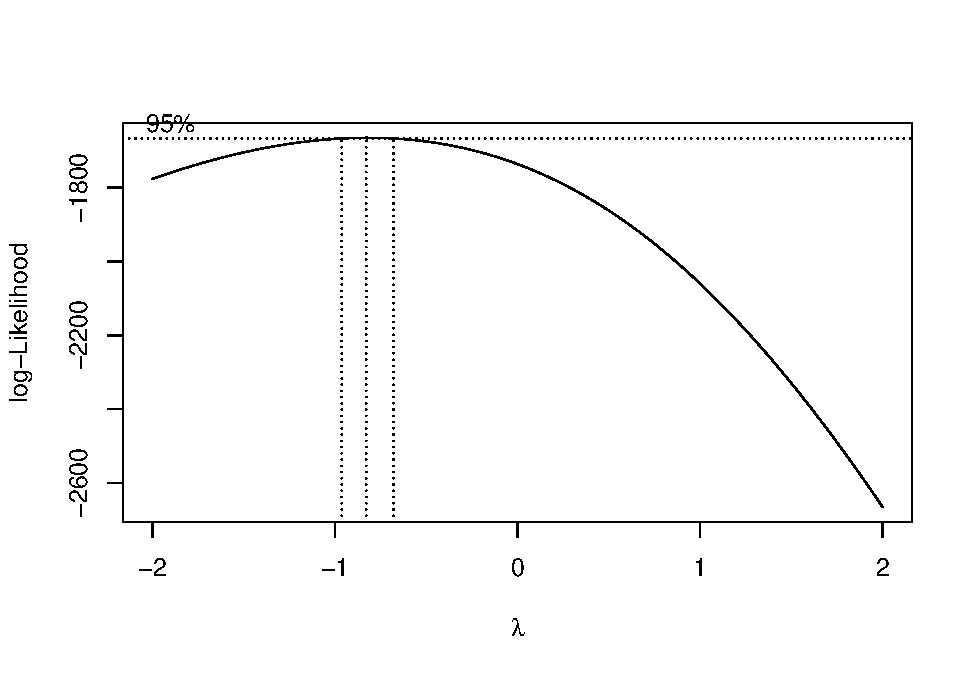
\includegraphics{01_CSI_online_aphasia_power_analysis_summary_files/figure-latex/RT distributions-1.pdf}

\begin{Shaded}
\begin{Highlighting}[]
\CommentTok{\# apply transformation}
\NormalTok{df\_Ord}\SpecialCharTok{$}\NormalTok{iRT }\OtherTok{\textless{}{-}}\DecValTok{1000}\SpecialCharTok{/}\NormalTok{df\_Ord}\SpecialCharTok{$}\NormalTok{RT}
\FunctionTok{plot}\NormalTok{(df\_Ord}\SpecialCharTok{$}\NormalTok{RT, df\_Ord}\SpecialCharTok{$}\NormalTok{iRT)}
\end{Highlighting}
\end{Shaded}

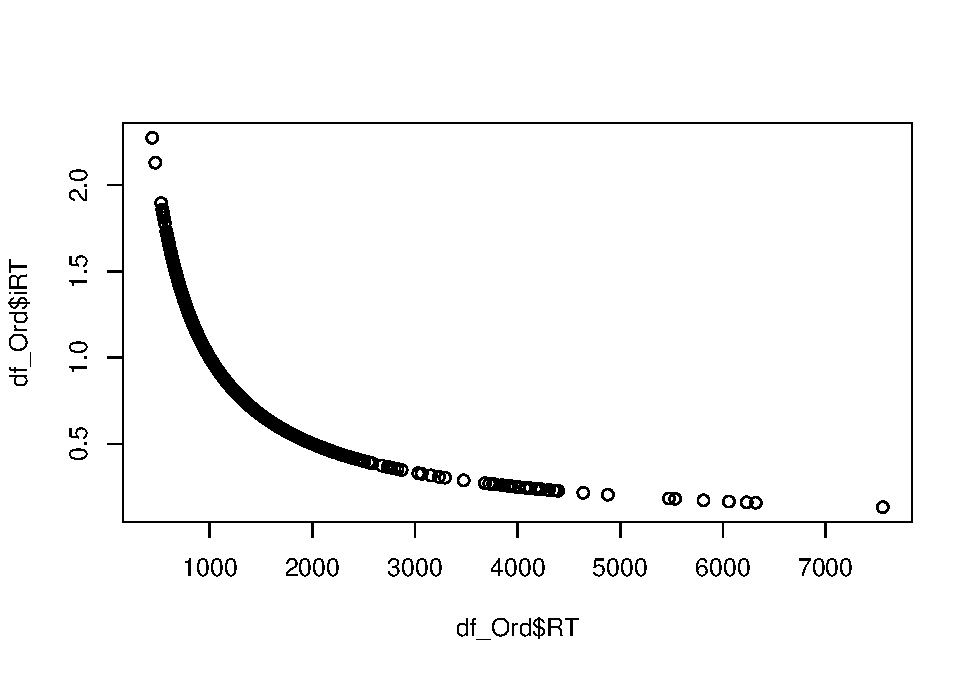
\includegraphics{01_CSI_online_aphasia_power_analysis_summary_files/figure-latex/RT distributions-2.pdf}

\begin{Shaded}
\begin{Highlighting}[]
\CommentTok{\# check fit}
\NormalTok{fit.normal\_inv}\OtherTok{\textless{}{-}}\NormalTok{ fitdistrplus}\SpecialCharTok{::}\FunctionTok{fitdist}\NormalTok{(df\_Ord}\SpecialCharTok{$}\NormalTok{iRT, }\AttributeTok{distr =} \StringTok{"norm"}\NormalTok{, }\AttributeTok{method =} \StringTok{"mle"}\NormalTok{)}
\FunctionTok{summary}\NormalTok{(fit.normal\_inv)}
\end{Highlighting}
\end{Shaded}

\begin{verbatim}
## Fitting of the distribution ' norm ' by maximum likelihood 
## Parameters : 
##       estimate  Std. Error
## mean 0.9329607 0.013612620
## sd   0.3588675 0.009625239
## Loglikelihood:  -273.9248   AIC:  551.8497   BIC:  560.9375 
## Correlation matrix:
##      mean sd
## mean    1  0
## sd      0  1
\end{verbatim}

\begin{Shaded}
\begin{Highlighting}[]
\FunctionTok{plot}\NormalTok{(fit.normal\_inv)}
\end{Highlighting}
\end{Shaded}

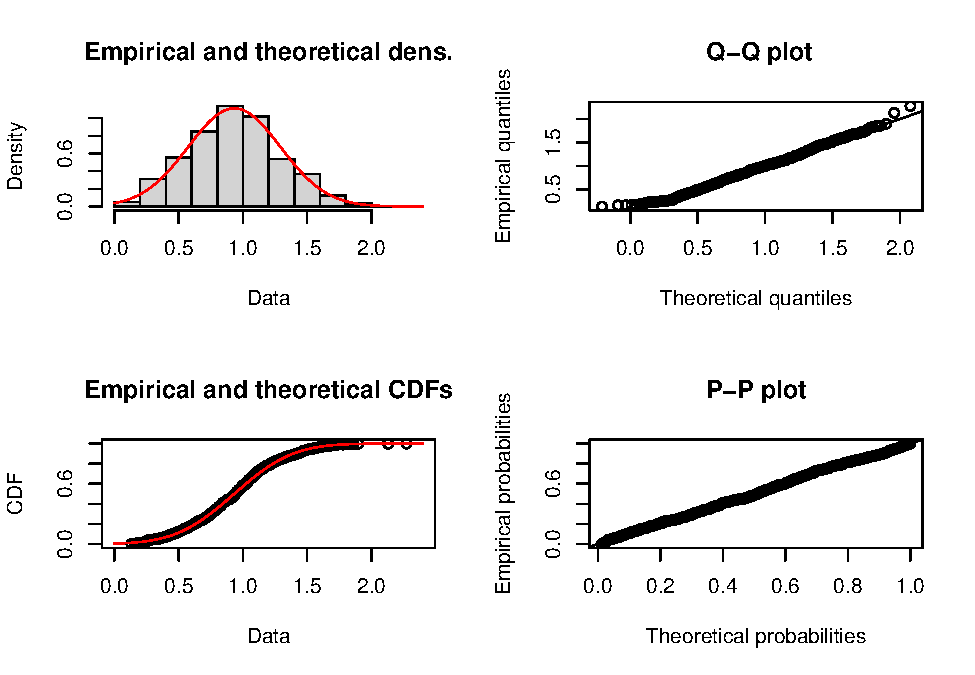
\includegraphics{01_CSI_online_aphasia_power_analysis_summary_files/figure-latex/RT distributions-3.pdf}

\begin{enumerate}
\def\labelenumi{\alph{enumi})}
\setcounter{enumi}{2}
\tightlist
\item
  Set up the model \emph{Model 1: Linear model with continuous predictor
  ``Ordinal position'' as the only predictor and inversely transformed
  RT data}
\end{enumerate}

\begin{Shaded}
\begin{Highlighting}[]
\NormalTok{lmm1 }\OtherTok{\textless{}{-}} \FunctionTok{lmer}\NormalTok{(iRT }\SpecialCharTok{\textasciitilde{}}\NormalTok{ OrdPos.c }\SpecialCharTok{+} 
\NormalTok{               (OrdPos.c}\SpecialCharTok{|}\NormalTok{subject) }\SpecialCharTok{+}\NormalTok{(OrdPos.c}\SpecialCharTok{|}\NormalTok{cat\_nr) ,}
            \AttributeTok{data =}\NormalTok{ df\_Ord, }\AttributeTok{REML =} \ConstantTok{FALSE}\NormalTok{,}
            \AttributeTok{control=}\FunctionTok{lmerControl}\NormalTok{(}\AttributeTok{optimizer =} \StringTok{"bobyqa"}\NormalTok{))}
\FunctionTok{isSingular}\NormalTok{(lmm1)}
\end{Highlighting}
\end{Shaded}

\begin{verbatim}
## [1] FALSE
\end{verbatim}

\begin{Shaded}
\begin{Highlighting}[]
\FunctionTok{summary}\NormalTok{(lmm1)}
\end{Highlighting}
\end{Shaded}

\begin{verbatim}
## Linear mixed model fit by maximum likelihood . t-tests use Satterthwaite's
##   method [lmerModLmerTest]
## Formula: iRT ~ OrdPos.c + (OrdPos.c | subject) + (OrdPos.c | cat_nr)
##    Data: df_Ord
## Control: lmerControl(optimizer = "bobyqa")
## 
##      AIC      BIC   logLik deviance df.resid 
##    354.3    395.2   -168.1    336.3      686 
## 
## Scaled residuals: 
##      Min       1Q   Median       3Q      Max 
## -2.94617 -0.64056  0.07423  0.61505  3.04551 
## 
## Random effects:
##  Groups   Name        Variance  Std.Dev. Corr 
##  subject  (Intercept) 0.0334551 0.18291       
##           OrdPos.c    0.0003164 0.01779  -0.58
##  cat_nr   (Intercept) 0.0106732 0.10331       
##           OrdPos.c    0.0003476 0.01864  -0.24
##  Residual             0.0840919 0.28999       
## Number of obs: 695, groups:  subject, 18; cat_nr, 17
## 
## Fixed effects:
##             Estimate Std. Error       df t value Pr(>|t|)    
## (Intercept)  0.92215    0.05157 25.89346  17.881 4.33e-16 ***
## OrdPos.c    -0.03048    0.01013 11.39100  -3.008   0.0115 *  
## ---
## Signif. codes:  0 '***' 0.001 '**' 0.01 '*' 0.05 '.' 0.1 ' ' 1
## 
## Correlation of Fixed Effects:
##          (Intr)
## OrdPos.c -0.259
\end{verbatim}

\hypertarget{extend-dataset}{%
\subsection{2) Extend dataset}\label{extend-dataset}}

We already know that we want 24 categories (we use the same stimuli as
in Stark, van Scherpenberg et al., 2021). So we extend along
categories.\\
Additionally, we also reduce along participants: Our power curve
suggested that 16 participants would be sufficient to achieve a power of
.80 based on the effect size from Lorenz et al., 2016.

\begin{Shaded}
\begin{Highlighting}[]
\NormalTok{lmm1\_2 }\OtherTok{\textless{}{-}} \FunctionTok{extend}\NormalTok{(lmm1, }\AttributeTok{along=}\StringTok{"cat\_nr"}\NormalTok{, }\AttributeTok{n=}\DecValTok{24}\NormalTok{)}
\CommentTok{\# m2data \textless{}{-} getData(lmm1\_2) }
\CommentTok{\# \#\# ok, data were indeed extended to n categories ;{-})}
\CommentTok{\# str(m2data)}
\CommentTok{\# str(df\_Ord)}
\end{Highlighting}
\end{Shaded}

\hypertarget{specify-effect-size-and-run-power-analysis}{%
\subsection{3) Specify effect size and run power
analysis}\label{specify-effect-size-and-run-power-analysis}}

We use the experimental effect size from Lorenz et al

\emph{Linear model with continuous predictor ``Ordinal position'' and
inversely transformed RT data}

\begin{Shaded}
\begin{Highlighting}[]
\NormalTok{PowerLMM\_OrdPos\_Lorenz }\OtherTok{\textless{}{-}} \FunctionTok{powerCurve}\NormalTok{(lmm1\_2, }\AttributeTok{along =} \StringTok{"subject"}\NormalTok{, }\AttributeTok{breaks=}\DecValTok{16}\NormalTok{, }\AttributeTok{test=}\FunctionTok{fixed}\NormalTok{(}\StringTok{"OrdPos.c"}\NormalTok{,}\StringTok{"t"}\NormalTok{), }\AttributeTok{nsim =}\NormalTok{ n\_iter) }\CommentTok{\# increase to nsim \textgreater{} 1000 for real test}
\FunctionTok{lastResult}\NormalTok{()}\SpecialCharTok{$}\NormalTok{warnings}
\FunctionTok{lastResult}\NormalTok{()}\SpecialCharTok{$}\NormalTok{errors}
\end{Highlighting}
\end{Shaded}

\begin{Shaded}
\begin{Highlighting}[]
\NormalTok{PowerLMM\_OrdPos\_Lorenz}
\end{Highlighting}
\end{Shaded}

\begin{verbatim}
## Power for predictor 'OrdPos.c', (95% confidence interval),
## by number of levels in subject:
##      16: 90.90% (88.94, 92.61) - 943 rows
## 
## Time elapsed: 0 h 3 m 59 s
\end{verbatim}

\hypertarget{use-effect-from-stark-van-scherpenberg-et-al.-2021}{%
\subsection{5) Use effect from Stark, van Scherpenberg et al.,
2021}\label{use-effect-from-stark-van-scherpenberg-et-al.-2021}}

Our effect size from a neurotypical sample in an online experiment was
smaller. We we take this effect on 16 participants + 25 \% (=20
participants), the power is substantially reduced.

\emph{Extend to 20 participants}

\begin{Shaded}
\begin{Highlighting}[]
\NormalTok{lmm24\_20\_Stark }\OtherTok{\textless{}{-}} \FunctionTok{extend}\NormalTok{(lmm1\_2, }\AttributeTok{along=}\StringTok{"subject"}\NormalTok{, }\AttributeTok{n=}\DecValTok{20}\NormalTok{)}
\CommentTok{\#str(lmm24\_20\_Stark)}
\end{Highlighting}
\end{Shaded}

\emph{Specify effect size}\\
What effect size is 31 ms in 1/(RT/1000) depends on the position: We
take the grand mean

\begin{Shaded}
\begin{Highlighting}[]
\CommentTok{\# calculate the effect size in the transformed scale}
\NormalTok{gm }\OtherTok{\textless{}{-}} \FunctionTok{mean}\NormalTok{(df\_Ord}\SpecialCharTok{$}\NormalTok{RT)}
\NormalTok{eff1 }\OtherTok{\textless{}{-}} \DecValTok{1000}\SpecialCharTok{/}\NormalTok{(gm}\SpecialCharTok{+}\NormalTok{(}\DecValTok{31}\SpecialCharTok{/}\DecValTok{2}\NormalTok{)) }\SpecialCharTok{{-}} \DecValTok{1000}\SpecialCharTok{/}\NormalTok{(gm}\SpecialCharTok{{-}}\NormalTok{(}\DecValTok{31}\SpecialCharTok{/}\DecValTok{2}\NormalTok{))}

\CommentTok{\# use this as the fixed effect of interest}
\FunctionTok{fixef}\NormalTok{(lmm24\_20\_Stark)[}\StringTok{"OrdPos.c"}\NormalTok{] }\OtherTok{\textless{}{-}}\NormalTok{ eff1}
\end{Highlighting}
\end{Shaded}

\emph{Power analysis: Linear model with continuous predictor ``Ordinal
position'' (effect size from Stark et al., 2021) and inversely
transformed RT data}

\begin{Shaded}
\begin{Highlighting}[]
\NormalTok{PowerLMM\_OrdPos\_Stark }\OtherTok{\textless{}{-}} 
  \FunctionTok{powerSim}\NormalTok{(lmm24\_20\_Stark, }\AttributeTok{test=}\FunctionTok{fixed}\NormalTok{(}\StringTok{"OrdPos.c"}\NormalTok{,}\StringTok{"t"}\NormalTok{), }\AttributeTok{nsim =}\NormalTok{ n\_iter) }\CommentTok{\# increase to nsim \textgreater{} 1000 for real test}
\FunctionTok{lastResult}\NormalTok{()}\SpecialCharTok{$}\NormalTok{warnings}
\FunctionTok{lastResult}\NormalTok{()}\SpecialCharTok{$}\NormalTok{errors}
\end{Highlighting}
\end{Shaded}

\begin{Shaded}
\begin{Highlighting}[]
\NormalTok{PowerLMM\_OrdPos\_Stark}
\end{Highlighting}
\end{Shaded}

\begin{verbatim}
## Power for predictor 'OrdPos.c', (95% confidence interval):
##       50.80% (47.65, 53.94)
## 
## Test: t-test with Satterthwaite degrees of freedom (package lmerTest)
##       Effect size for OrdPos.c is -0.017
## 
## Based on 1000 simulations, (5 warnings, 0 errors)
## alpha = 0.05, nrow = 1193
## 
## Time elapsed: 0 h 4 m 46 s
\end{verbatim}

Unfortunately, if the effect was that small and the variance estimates
realistic, the power would be too low to reliably detect the effect. A
power curve suggests that the power would still be below 80 \% with 60
participants. Thus, this seems to be a risk that we need to take.
Moreover, our main interest is the analyis across the three sessions.

\hypertarget{section}{%
\section{--------------------------------------------}\label{section}}

\hypertarget{comparison-2-power-analysis-for-the-ordinal-position-effect-across-all-three-sessions-ordinal-position-and-interaction-effect}{%
\section{Comparison 2: Power analysis for the ordinal position effect
across all three sessions (Ordinal position and interaction
effect)}\label{comparison-2-power-analysis-for-the-ordinal-position-effect-across-all-three-sessions-ordinal-position-and-interaction-effect}}

As a proxy for our sessions, we will use the variances from the three
repetitions of the first session in Lorenz et al (2021)

Subset the data to the first session

\begin{Shaded}
\begin{Highlighting}[]
\NormalTok{df\_full }\OtherTok{\textless{}{-}}\NormalTok{ df }\SpecialCharTok{\%\textgreater{}\%} \FunctionTok{filter}\NormalTok{(wh }\SpecialCharTok{==} \DecValTok{1}\NormalTok{) }\SpecialCharTok{\%\textgreater{}\%} \FunctionTok{droplevels}\NormalTok{()}
\end{Highlighting}
\end{Shaded}

\hypertarget{set-up-models-based-on-the-structure-of-the-new-experiment}{%
\subsection{1) Set up models based on the structure of the new
experiment}\label{set-up-models-based-on-the-structure-of-the-new-experiment}}

Unfortunately, simr does not work properly with GLMMs. Therefore, for
the power analysis, we will set up an LMM with transformed RTs\\
a) center OrdPos (continuous predictor)

\begin{Shaded}
\begin{Highlighting}[]
\CommentTok{\# center continuous predictor}
\NormalTok{df\_full }\SpecialCharTok{\%\textgreater{}\%} \FunctionTok{mutate}\NormalTok{(}\AttributeTok{OrdPos\_num =} \FunctionTok{case\_when}\NormalTok{(OrdPos }\SpecialCharTok{==} \StringTok{"OP1"} \SpecialCharTok{\textasciitilde{}}\DecValTok{1}\NormalTok{,}
\NormalTok{                                         OrdPos }\SpecialCharTok{==} \StringTok{"OP2"} \SpecialCharTok{\textasciitilde{}}\DecValTok{2}\NormalTok{,}
\NormalTok{                                         OrdPos }\SpecialCharTok{==} \StringTok{"OP3"} \SpecialCharTok{\textasciitilde{}}\DecValTok{3}\NormalTok{,}
\NormalTok{                                         OrdPos }\SpecialCharTok{==} \StringTok{"OP4"} \SpecialCharTok{\textasciitilde{}}\DecValTok{4}\NormalTok{,}
\NormalTok{                                         OrdPos }\SpecialCharTok{==} \StringTok{"OP5"} \SpecialCharTok{\textasciitilde{}}\DecValTok{5}\NormalTok{)) }\SpecialCharTok{\%\textgreater{}\%}
                  \FunctionTok{mutate}\NormalTok{(}\AttributeTok{OrdPos.c=}
                    \FunctionTok{scale}\NormalTok{(}\FunctionTok{as.numeric}\NormalTok{(}\FunctionTok{as.character}\NormalTok{(OrdPos\_num)), }
                     \AttributeTok{center =} \ConstantTok{TRUE}\NormalTok{, }\AttributeTok{scale =} \ConstantTok{FALSE}\NormalTok{)) }\OtherTok{{-}\textgreater{}}\NormalTok{ df\_full}
\end{Highlighting}
\end{Shaded}

\begin{enumerate}
\def\labelenumi{\alph{enumi})}
\setcounter{enumi}{1}
\tightlist
\item
  Check distribution of RTs: An inverse transformation (1000/x) is
  needed and appropriate
\end{enumerate}

\begin{Shaded}
\begin{Highlighting}[]
\CommentTok{\# Boxcox plot suggests inverse transformation: }
\FunctionTok{boxcox}\NormalTok{(df\_full}\SpecialCharTok{$}\NormalTok{RT }\SpecialCharTok{\textasciitilde{}}\NormalTok{ df\_full}\SpecialCharTok{$}\NormalTok{OrdPos)}
\end{Highlighting}
\end{Shaded}

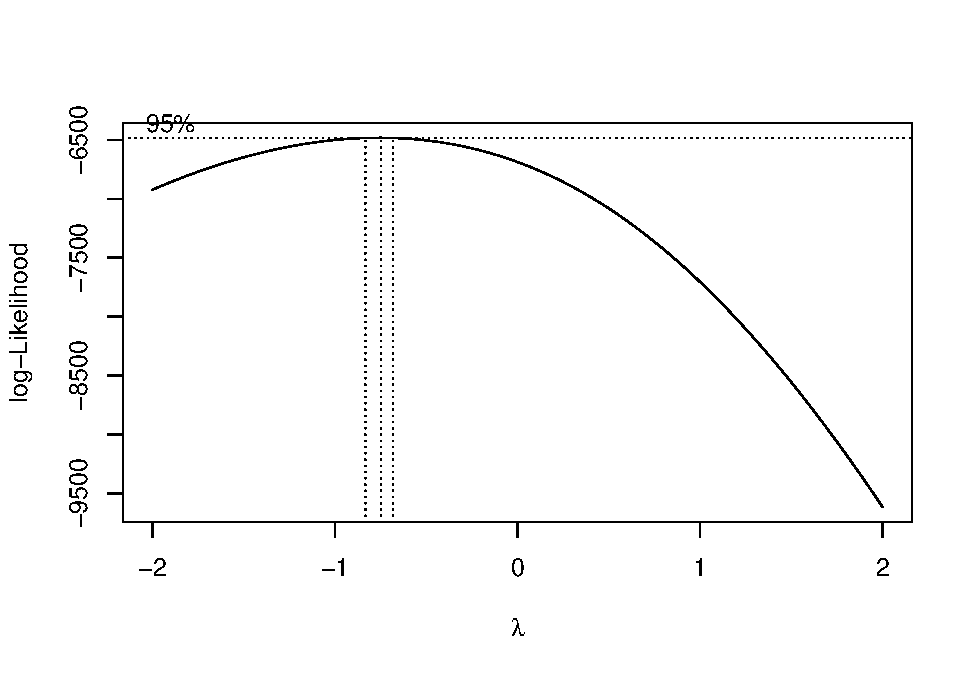
\includegraphics{01_CSI_online_aphasia_power_analysis_summary_files/figure-latex/RT distributions2-1.pdf}

\begin{Shaded}
\begin{Highlighting}[]
\CommentTok{\# apply transformation}
\NormalTok{df\_full}\SpecialCharTok{$}\NormalTok{iRT }\OtherTok{\textless{}{-}}\DecValTok{1000}\SpecialCharTok{/}\NormalTok{df\_full}\SpecialCharTok{$}\NormalTok{RT}
\FunctionTok{plot}\NormalTok{(df\_full}\SpecialCharTok{$}\NormalTok{RT, df\_full}\SpecialCharTok{$}\NormalTok{iRT)}
\end{Highlighting}
\end{Shaded}

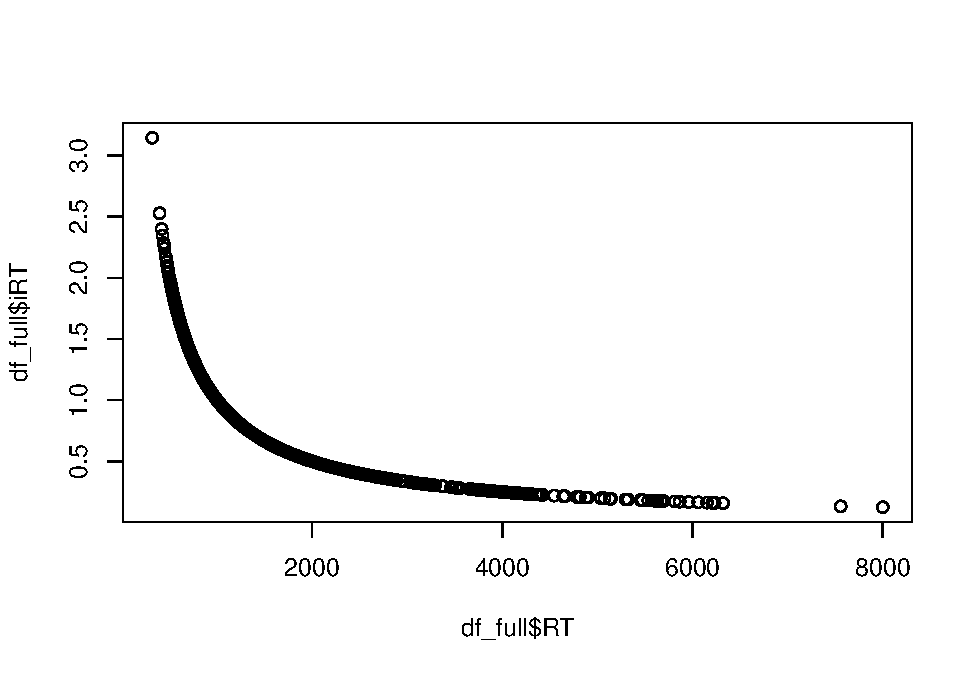
\includegraphics{01_CSI_online_aphasia_power_analysis_summary_files/figure-latex/RT distributions2-2.pdf}

\begin{Shaded}
\begin{Highlighting}[]
\CommentTok{\# check fit}
\NormalTok{fit.normal\_inv}\OtherTok{\textless{}{-}}\NormalTok{ fitdistrplus}\SpecialCharTok{::}\FunctionTok{fitdist}\NormalTok{(df\_full}\SpecialCharTok{$}\NormalTok{iRT, }\AttributeTok{distr =} \StringTok{"norm"}\NormalTok{, }\AttributeTok{method =} \StringTok{"mle"}\NormalTok{)}
\FunctionTok{summary}\NormalTok{(fit.normal\_inv)}
\end{Highlighting}
\end{Shaded}

\begin{verbatim}
## Fitting of the distribution ' norm ' by maximum likelihood 
## Parameters : 
##       estimate  Std. Error
## mean 0.9781205 0.008345432
## sd   0.3879504 0.005900935
## Loglikelihood:  -1020.123   AIC:  2044.246   BIC:  2055.603 
## Correlation matrix:
##      mean sd
## mean    1  0
## sd      0  1
\end{verbatim}

\begin{Shaded}
\begin{Highlighting}[]
\FunctionTok{plot}\NormalTok{(fit.normal\_inv)}
\end{Highlighting}
\end{Shaded}

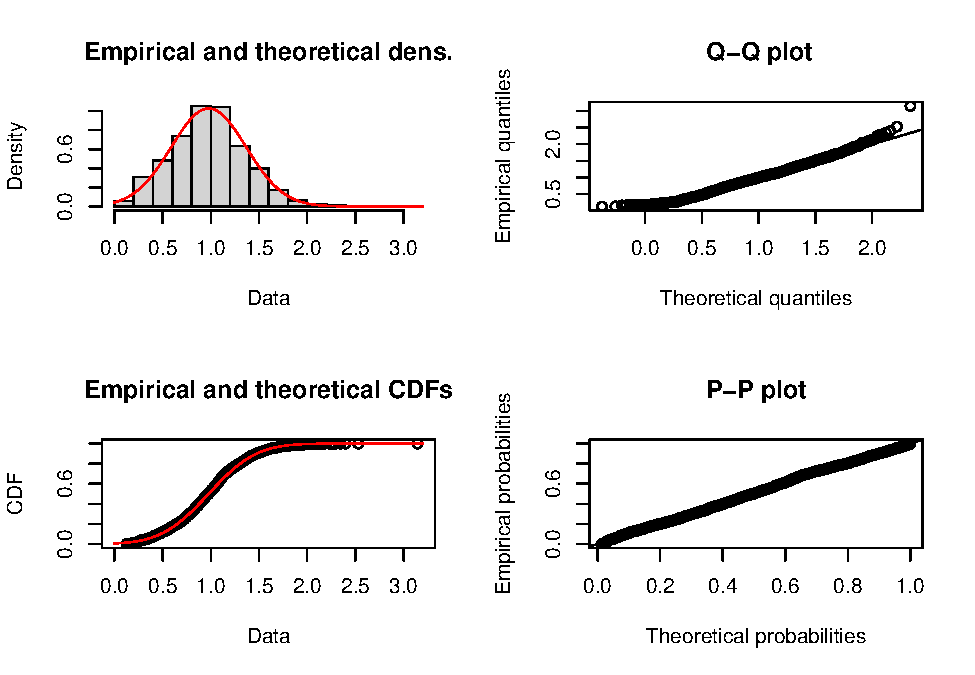
\includegraphics{01_CSI_online_aphasia_power_analysis_summary_files/figure-latex/RT distributions2-3.pdf}

\begin{enumerate}
\def\labelenumi{\alph{enumi})}
\setcounter{enumi}{2}
\tightlist
\item
  Set up the model \emph{Linear model with continuous predictor
  ``Ordinal position'' and fatcor ``repet'' (sliding difference
  contrast) as the predictor variables and inversely transformed RT
  data}
\end{enumerate}

\begin{Shaded}
\begin{Highlighting}[]
\CommentTok{\# compute sliding difference contrast: Intercept is grand mean, second level is compared to first level}
\FunctionTok{contrasts}\NormalTok{(df\_full}\SpecialCharTok{$}\NormalTok{repet) }\OtherTok{\textless{}{-}} \FunctionTok{contr.sdif}\NormalTok{(}\DecValTok{3}\NormalTok{)}
\CommentTok{\# maximal model has singular fit {-} stepwise reduction}
\CommentTok{\# lmm1 \textless{}{-} lmer(iRT \textasciitilde{} OrdPos.c*repet +}
\CommentTok{\#               (OrdPos.c*repet|subject) +(OrdPos.c*repet|cat\_nr) ,}
\CommentTok{\#            data = df\_full, REML = FALSE,}
\CommentTok{\#            control=lmerControl(optimizer = "bobyqa"))}

\NormalTok{lmm1 }\OtherTok{\textless{}{-}}\NormalTok{ afex}\SpecialCharTok{::}\FunctionTok{lmer\_alt}\NormalTok{(iRT }\SpecialCharTok{\textasciitilde{}}\NormalTok{ OrdPos.c}\SpecialCharTok{*}\NormalTok{repet }\SpecialCharTok{+}
\NormalTok{               (repet}\SpecialCharTok{||}\NormalTok{subject) }\SpecialCharTok{+}\NormalTok{(OrdPos.c}\SpecialCharTok{||}\NormalTok{cat\_nr) ,}
            \AttributeTok{data =}\NormalTok{ df\_full, }\AttributeTok{REML =} \ConstantTok{FALSE}\NormalTok{,}
            \AttributeTok{control=}\FunctionTok{lmerControl}\NormalTok{(}\AttributeTok{optimizer =} \StringTok{"bobyqa"}\NormalTok{,}
                                \AttributeTok{optCtrl=}\FunctionTok{list}\NormalTok{(}\AttributeTok{maxfun=}\FloatTok{2e5}\NormalTok{)))}
\FunctionTok{isSingular}\NormalTok{(lmm1)}
\end{Highlighting}
\end{Shaded}

\begin{verbatim}
## [1] FALSE
\end{verbatim}

\begin{Shaded}
\begin{Highlighting}[]
\FunctionTok{summary}\NormalTok{(lmm1)}
\end{Highlighting}
\end{Shaded}

\begin{verbatim}
## Linear mixed model fit by maximum likelihood . t-tests use Satterthwaite's
##   method [lmerModLmerTest]
## Formula: iRT ~ OrdPos.c * repet + (1 + re1.repet2.1 + re1.repet3.2 ||  
##     subject) + (1 + re2.OrdPos.c || cat_nr)
##    Data: data
## Control: lmerControl(optimizer = "bobyqa", optCtrl = list(maxfun = 2e+05))
## 
##      AIC      BIC   logLik deviance df.resid 
##   1139.4   1207.5   -557.7   1115.4     2149 
## 
## Scaled residuals: 
##     Min      1Q  Median      3Q     Max 
## -3.2704 -0.6453  0.0760  0.6398  5.1565 
## 
## Random effects:
##  Groups    Name         Variance  Std.Dev.
##  subject   (Intercept)  0.0457486 0.21389 
##  subject.1 re1.repet2.1 0.0011736 0.03426 
##  subject.2 re1.repet3.2 0.0006358 0.02522 
##  cat_nr    (Intercept)  0.0138004 0.11748 
##  cat_nr.1  re2.OrdPos.c 0.0001398 0.01182 
##  Residual               0.0922992 0.30381 
## Number of obs: 2161, groups:  subject, 18; cat_nr, 17
## 
## Fixed effects:
##                     Estimate Std. Error         df t value Pr(>|t|)    
## (Intercept)        9.488e-01  5.848e-02  2.721e+01  16.223 1.62e-15 ***
## OrdPos.c          -1.976e-02  5.580e-03  1.681e+01  -3.541  0.00255 ** 
## repet2-1           5.028e-02  1.806e-02  2.069e+01   2.785  0.01120 *  
## repet3-2           4.273e-02  1.696e-02  2.002e+01   2.520  0.02034 *  
## OrdPos.c:repet2-1  1.442e-02  1.136e-02  2.094e+03   1.269  0.20449    
## OrdPos.c:repet3-2  3.068e-03  1.117e-02  2.092e+03   0.275  0.78359    
## ---
## Signif. codes:  0 '***' 0.001 '**' 0.01 '*' 0.05 '.' 0.1 ' ' 1
## 
## Correlation of Fixed Effects:
##             (Intr) OrdPs. rpt2-1 rpt3-2 OP.:2-
## OrdPos.c     0.000                            
## repet2-1    -0.002 -0.004                     
## repet3-2    -0.001 -0.004 -0.415              
## OrdPs.c:2-1 -0.001 -0.014  0.007  0.000       
## OrdPs.c:3-2 -0.001 -0.009  0.000 -0.007 -0.499
\end{verbatim}

\hypertarget{extend-dataset-1}{%
\subsection{2) Extend dataset}\label{extend-dataset-1}}

We already know that we want 24 categories (we use the same stimuli as
in Stark, van Scherpenberg et al., 2021). So we extend along
categories.\\
Additionally, we also reduce along participants: Our power curve
suggested that 16 participants would be sufficient to achieve a power of
.80 based on the effect size from Lorenz et al., 2016.

\begin{Shaded}
\begin{Highlighting}[]
\NormalTok{lmm1\_2 }\OtherTok{\textless{}{-}} \FunctionTok{extend}\NormalTok{(lmm1, }\AttributeTok{along=}\StringTok{"cat\_nr"}\NormalTok{, }\AttributeTok{n=}\DecValTok{24}\NormalTok{)}
\CommentTok{\# m2data \textless{}{-} getData(lmm1\_2) }
\CommentTok{\# \#\# ok, data were indeed extended to n categories ;{-})}
\CommentTok{\# str(m2data)}
\CommentTok{\# str(df\_full)}
\end{Highlighting}
\end{Shaded}

\hypertarget{specify-effect-size-and-run-power-analysis-1}{%
\subsection{3) Specify effect size and run power
analysis}\label{specify-effect-size-and-run-power-analysis-1}}

We use the experimental effect size from Lorenz et al to see the power
if all effects remained the same

\emph{Linear model with continuous predictor ``Ordinal position'',
sliding difference contrasted predictor repetition and inversely
transformed RT data}

\begin{Shaded}
\begin{Highlighting}[]
\NormalTok{PowerLMM\_OrdPos\_Lorenz }\OtherTok{\textless{}{-}} \FunctionTok{powerCurve}\NormalTok{(lmm1\_2, }\AttributeTok{along =} \StringTok{"subject"}\NormalTok{, }\AttributeTok{breaks=}\DecValTok{16}\NormalTok{, }\AttributeTok{test=}\FunctionTok{fixed}\NormalTok{(}\StringTok{"OrdPos.c"}\NormalTok{,}\StringTok{"t"}\NormalTok{), }\AttributeTok{nsim =}\NormalTok{ n\_iter) }\CommentTok{\# increase to nsim \textgreater{} 1000 for real test}
\FunctionTok{lastResult}\NormalTok{()}\SpecialCharTok{$}\NormalTok{warnings}
\FunctionTok{lastResult}\NormalTok{()}\SpecialCharTok{$}\NormalTok{errors}
\end{Highlighting}
\end{Shaded}

\begin{Shaded}
\begin{Highlighting}[]
\NormalTok{PowerLMM\_OrdPos\_Lorenz}
\end{Highlighting}
\end{Shaded}

\begin{verbatim}
## Power for predictor 'OrdPos.c', (95% confidence interval),
## by number of levels in subject:
##      16: 98.20% (97.17, 98.93) - 2906 rows
## 
## Time elapsed: 0 h 14 m 41 s
\end{verbatim}

\hypertarget{use-effect-from-stark-van-scherpenberg-et-al.-2021-1}{%
\subsection{5) Use effect from Stark, van Scherpenberg et al.,
2021}\label{use-effect-from-stark-van-scherpenberg-et-al.-2021-1}}

Our effect size from a neurotypical sample in an online experiment was
smaller. We take this effect on 16 participants + 25 \% (=20
participants), the power is substantially reduced.

\emph{Extend to 20 participants}

\begin{Shaded}
\begin{Highlighting}[]
\NormalTok{lmm24\_20\_Stark }\OtherTok{\textless{}{-}} \FunctionTok{extend}\NormalTok{(lmm1\_2, }\AttributeTok{along=}\StringTok{"subject"}\NormalTok{, }\AttributeTok{n=}\DecValTok{20}\NormalTok{)}
\CommentTok{\#str(lmm24\_20\_Stark)}
\end{Highlighting}
\end{Shaded}

\emph{Specifiy effect size}\\
What effect size is 31 ms in 1/(RT/1000) depends on the position: We
take the grand mean

\begin{Shaded}
\begin{Highlighting}[]
\CommentTok{\# calculate the effect size in the transformed scale}
\NormalTok{gm }\OtherTok{\textless{}{-}} \FunctionTok{mean}\NormalTok{(df\_Ord}\SpecialCharTok{$}\NormalTok{RT)}
\NormalTok{eff1 }\OtherTok{\textless{}{-}} \DecValTok{1000}\SpecialCharTok{/}\NormalTok{(gm}\SpecialCharTok{+}\NormalTok{(}\DecValTok{31}\SpecialCharTok{/}\DecValTok{2}\NormalTok{)) }\SpecialCharTok{{-}} \DecValTok{1000}\SpecialCharTok{/}\NormalTok{(gm}\SpecialCharTok{{-}}\NormalTok{(}\DecValTok{31}\SpecialCharTok{/}\DecValTok{2}\NormalTok{))}

\CommentTok{\# use this as the fixed effect of interest}
\FunctionTok{fixef}\NormalTok{(lmm24\_20\_Stark)[}\StringTok{"OrdPos.c"}\NormalTok{] }\OtherTok{\textless{}{-}}\NormalTok{ eff1}
\end{Highlighting}
\end{Shaded}

\emph{Power analysis: Linear model with continuous predictor ``Ordinal
position'' (effect size from Stark et al., 2021) and inversely
transformed RT data}

\begin{Shaded}
\begin{Highlighting}[]
\NormalTok{PowerLMM\_OrdPos\_Stark }\OtherTok{\textless{}{-}} 
  \FunctionTok{powerSim}\NormalTok{(lmm24\_20\_Stark, }\AttributeTok{test=}\FunctionTok{fixed}\NormalTok{(}\StringTok{"OrdPos.c"}\NormalTok{,}\StringTok{"t"}\NormalTok{), }\AttributeTok{nsim =}\NormalTok{ n\_iter) }\CommentTok{\# increase to nsim \textgreater{} 1000 for real test}
\FunctionTok{lastResult}\NormalTok{()}\SpecialCharTok{$}\NormalTok{warnings}
\FunctionTok{lastResult}\NormalTok{()}\SpecialCharTok{$}\NormalTok{errors}
\end{Highlighting}
\end{Shaded}

\begin{Shaded}
\begin{Highlighting}[]
\NormalTok{PowerLMM\_OrdPos\_Stark}
\end{Highlighting}
\end{Shaded}

\begin{verbatim}
## Power for predictor 'OrdPos.c', (95% confidence interval):
##       97.50% (96.33, 98.38)
## 
## Test: t-test with Satterthwaite degrees of freedom (package lmerTest)
##       Effect size for OrdPos.c is -0.017
## 
## Based on 1000 simulations, (6 warnings, 0 errors)
## alpha = 0.05, nrow = 3685
## 
## Time elapsed: 0 h 17 m 44 s
\end{verbatim}

Now, the power is high even with the more conservative effect size
estimate.

\hypertarget{estimate-the-effect-size-of-the-interaction-effect-of-the-ordinal-position-x-session-we-can-reliably-detect-with-our-20-vp---with-oridnal-position-effect-from-lorenz-et-al-2021}{%
\subsection{6) Estimate the effect size of the interaction effect of the
ordinal position x Session we can reliably detect with our 20 VP - with
oridnal position effect from Lorenz et al
(2021)}\label{estimate-the-effect-size-of-the-interaction-effect-of-the-ordinal-position-x-session-we-can-reliably-detect-with-our-20-vp---with-oridnal-position-effect-from-lorenz-et-al-2021}}

\hypertarget{extend-data-set}{%
\subsection{Extend data set}\label{extend-data-set}}

\begin{Shaded}
\begin{Highlighting}[]
\NormalTok{lmm1\_2 }\OtherTok{\textless{}{-}} \FunctionTok{extend}\NormalTok{(lmm1, }\AttributeTok{along=}\StringTok{"cat\_nr"}\NormalTok{, }\AttributeTok{n=}\DecValTok{24}\NormalTok{)}
\NormalTok{lmm24\_20 }\OtherTok{\textless{}{-}} \FunctionTok{extend}\NormalTok{(lmm1, }\AttributeTok{along=}\StringTok{"subject"}\NormalTok{, }\AttributeTok{n=}\DecValTok{20}\NormalTok{)}
\end{Highlighting}
\end{Shaded}

\hypertarget{specify-effect-sizes-and-run-different-power-analyses}{%
\subsubsection{Specify effect sizes and run different power
analyses}\label{specify-effect-sizes-and-run-different-power-analyses}}

To specify the effect sizes, we always take the grand mean and take +-
1/2 the inversely transformed difference we want to implement. We keep
the two main effects unchanged.

\hypertarget{ms-interaction-effect-20-vp}{%
\paragraph{40 ms interaction effect, 20
VP}\label{ms-interaction-effect-20-vp}}

\begin{Shaded}
\begin{Highlighting}[]
\NormalTok{gm }\OtherTok{\textless{}{-}} \FunctionTok{mean}\NormalTok{(df\_Ord}\SpecialCharTok{$}\NormalTok{RT)}
\NormalTok{eff\_40ms }\OtherTok{\textless{}{-}}\NormalTok{ (}\DecValTok{1000}\SpecialCharTok{/}\NormalTok{(gm}\SpecialCharTok{+}\NormalTok{(}\DecValTok{40}\SpecialCharTok{/}\DecValTok{2}\NormalTok{))) }\SpecialCharTok{{-}}\NormalTok{ (}\DecValTok{1000}\SpecialCharTok{/}\NormalTok{(gm}\SpecialCharTok{{-}}\NormalTok{(}\DecValTok{40}\SpecialCharTok{/}\DecValTok{2}\NormalTok{)))}
\FunctionTok{fixef}\NormalTok{(lmm24\_20\_Stark)[}\StringTok{"OrdPos.c:repet2{-}1"}\NormalTok{]}\OtherTok{\textless{}{-}}\NormalTok{ eff\_40ms}
\FunctionTok{fixef}\NormalTok{(lmm24\_20\_Stark)[}\StringTok{"OrdPos.c:repet3{-}2"}\NormalTok{]}\OtherTok{\textless{}{-}}\NormalTok{ eff\_40ms}
\end{Highlighting}
\end{Shaded}

\emph{Model B2: Linear model with interaction effect ``Ordinal position
x Session'' of 40 ms and ordinal position effect from Stark et al.,
2021}

\begin{Shaded}
\begin{Highlighting}[]
\NormalTok{PowerLMM1\_Interaction24\_20\_Stark }\OtherTok{\textless{}{-}} \FunctionTok{powerSim}\NormalTok{(lmm24\_20\_Stark, }\AttributeTok{test=}\FunctionTok{fixed}\NormalTok{(}\StringTok{"OrdPos.c:repet2{-}1"}\NormalTok{,}\StringTok{"t"}\NormalTok{), }\AttributeTok{nsim =}\NormalTok{ n\_iter) }\CommentTok{\# increase to nsim \textgreater{} 1000 for real test}
\FunctionTok{lastResult}\NormalTok{()}\SpecialCharTok{$}\NormalTok{warnings}
\FunctionTok{lastResult}\NormalTok{()}\SpecialCharTok{$}\NormalTok{errors}
\end{Highlighting}
\end{Shaded}

\begin{Shaded}
\begin{Highlighting}[]
\NormalTok{PowerLMM1\_Interaction24\_20\_Stark}
\end{Highlighting}
\end{Shaded}

\begin{verbatim}
## Power for predictor 'OrdPos.c:repet2-1', (95% confidence interval):
##       72.80% (69.93, 75.54)
## 
## Test: t-test with Satterthwaite degrees of freedom (package lmerTest)
##       Effect size for OrdPos.c:repet2-1 is -0.022
## 
## Based on 1000 simulations, (12 warnings, 0 errors)
## alpha = 0.05, nrow = 3685
## 
## Time elapsed: 0 h 17 m 56 s
\end{verbatim}

\begin{Shaded}
\begin{Highlighting}[]
\NormalTok{PowerLMM1\_Interaction24\_20\_Stark }\OtherTok{\textless{}{-}} \FunctionTok{powerSim}\NormalTok{(lmm24\_20\_Stark, }\AttributeTok{test=}\FunctionTok{fixed}\NormalTok{(}\StringTok{"OrdPos.c:repet3{-}2"}\NormalTok{,}\StringTok{"t"}\NormalTok{), }\AttributeTok{nsim =}\NormalTok{ n\_iter) }\CommentTok{\# increase to nsim \textgreater{} 1000 for real test}
\FunctionTok{lastResult}\NormalTok{()}\SpecialCharTok{$}\NormalTok{warnings}
\FunctionTok{lastResult}\NormalTok{()}\SpecialCharTok{$}\NormalTok{errors}
\end{Highlighting}
\end{Shaded}

\begin{Shaded}
\begin{Highlighting}[]
\NormalTok{PowerLMM1\_Interaction24\_20\_Stark}
\end{Highlighting}
\end{Shaded}

\begin{verbatim}
## Power for predictor 'OrdPos.c:repet3-2', (95% confidence interval):
##       74.70% (71.89, 77.37)
## 
## Test: t-test with Satterthwaite degrees of freedom (package lmerTest)
##       Effect size for OrdPos.c:repet3-2 is -0.022
## 
## Based on 1000 simulations, (9 warnings, 0 errors)
## alpha = 0.05, nrow = 3685
## 
## Time elapsed: 0 h 17 m 49 s
\end{verbatim}

\hypertarget{ms-interaction-effect-20-vp-1}{%
\paragraph{45 ms interaction effect, 20
VP}\label{ms-interaction-effect-20-vp-1}}

\begin{Shaded}
\begin{Highlighting}[]
\NormalTok{gm }\OtherTok{\textless{}{-}} \FunctionTok{mean}\NormalTok{(df\_Ord}\SpecialCharTok{$}\NormalTok{RT)}
\NormalTok{eff\_45ms }\OtherTok{\textless{}{-}}\NormalTok{ (}\DecValTok{1000}\SpecialCharTok{/}\NormalTok{(gm}\SpecialCharTok{+}\NormalTok{(}\DecValTok{45}\SpecialCharTok{/}\DecValTok{2}\NormalTok{))) }\SpecialCharTok{{-}}\NormalTok{ (}\DecValTok{1000}\SpecialCharTok{/}\NormalTok{(gm}\SpecialCharTok{{-}}\NormalTok{(}\DecValTok{45}\SpecialCharTok{/}\DecValTok{2}\NormalTok{)))}
\FunctionTok{fixef}\NormalTok{(lmm24\_20\_Stark)[}\StringTok{"OrdPos.c:repet2{-}1"}\NormalTok{]}\OtherTok{\textless{}{-}}\NormalTok{ eff\_45ms}
\FunctionTok{fixef}\NormalTok{(lmm24\_20\_Stark)[}\StringTok{"OrdPos.c:repet3{-}2"}\NormalTok{]}\OtherTok{\textless{}{-}}\NormalTok{ eff\_45ms}
\end{Highlighting}
\end{Shaded}

\emph{Model B3: Linear model with interaction effect ``Ordinal position
x Session'' of 50 ms}

\begin{Shaded}
\begin{Highlighting}[]
\NormalTok{PowerLMM1\_Interaction45\_20 }\OtherTok{\textless{}{-}} \FunctionTok{powerSim}\NormalTok{(lmm24\_20, }\AttributeTok{test=}\FunctionTok{fixed}\NormalTok{(}\StringTok{"OrdPos.c:repet2{-}1"}\NormalTok{,}\StringTok{"t"}\NormalTok{), }\AttributeTok{nsim =}\NormalTok{ n\_iter) }\CommentTok{\# increase to nsim \textgreater{} 1000 for real test}
\FunctionTok{lastResult}\NormalTok{()}\SpecialCharTok{$}\NormalTok{warnings}
\FunctionTok{lastResult}\NormalTok{()}\SpecialCharTok{$}\NormalTok{errors}
\end{Highlighting}
\end{Shaded}

\begin{Shaded}
\begin{Highlighting}[]
\NormalTok{PowerLMM1\_Interaction45\_20}
\end{Highlighting}
\end{Shaded}

\begin{verbatim}
## Power for predictor 'OrdPos.c:repet2-1', (95% confidence interval):
##       63.80% (60.73, 66.78)
## 
## Test: t-test with Satterthwaite degrees of freedom (package lmerTest)
##       Effect size for OrdPos.c:repet2-1 is -0.025
## 
## Based on 1000 simulations, (6 warnings, 0 errors)
## alpha = 0.05, nrow = 2391
## 
## Time elapsed: 0 h 11 m 50 s
\end{verbatim}

\begin{Shaded}
\begin{Highlighting}[]
\NormalTok{PowerLMM1\_Interaction45\_20 }\OtherTok{\textless{}{-}} \FunctionTok{powerSim}\NormalTok{(lmm24\_20, }\AttributeTok{test=}\FunctionTok{fixed}\NormalTok{(}\StringTok{"OrdPos.c:repet3{-}2"}\NormalTok{,}\StringTok{"t"}\NormalTok{), }\AttributeTok{nsim =}\NormalTok{ n\_iter) }\CommentTok{\# increase to nsim \textgreater{} 1000 for real test}
\FunctionTok{lastResult}\NormalTok{()}\SpecialCharTok{$}\NormalTok{warnings}
\FunctionTok{lastResult}\NormalTok{()}\SpecialCharTok{$}\NormalTok{errors}
\end{Highlighting}
\end{Shaded}

\begin{Shaded}
\begin{Highlighting}[]
\NormalTok{PowerLMM1\_Interaction45\_20}
\end{Highlighting}
\end{Shaded}

\begin{verbatim}
## Power for predictor 'OrdPos.c:repet3-2', (95% confidence interval):
##       65.10% (62.05, 68.06)
## 
## Test: t-test with Satterthwaite degrees of freedom (package lmerTest)
##       Effect size for OrdPos.c:repet3-2 is -0.025
## 
## Based on 1000 simulations, (5 warnings, 0 errors)
## alpha = 0.05, nrow = 2391
## 
## Time elapsed: 0 h 11 m 48 s
\end{verbatim}

\emph{Model B4: Linear model with interaction effect ``Ordinal position
x Session'' of 45 ms and ordinal position effect from Stark et al.,
2021}

\begin{Shaded}
\begin{Highlighting}[]
\NormalTok{PowerLMM1\_Interaction45\_20\_Stark }\OtherTok{\textless{}{-}} \FunctionTok{powerSim}\NormalTok{(lmm24\_20\_Stark, }\AttributeTok{test=}\FunctionTok{fixed}\NormalTok{(}\StringTok{"OrdPos.c:repet2{-}1"}\NormalTok{,}\StringTok{"t"}\NormalTok{), }\AttributeTok{nsim =}\NormalTok{ n\_iter) }\CommentTok{\# increase to nsim \textgreater{} 1000 for real test}
\FunctionTok{lastResult}\NormalTok{()}\SpecialCharTok{$}\NormalTok{warnings}
\FunctionTok{lastResult}\NormalTok{()}\SpecialCharTok{$}\NormalTok{errors}
\end{Highlighting}
\end{Shaded}

\begin{Shaded}
\begin{Highlighting}[]
\NormalTok{PowerLMM1\_Interaction45\_20\_Stark}
\end{Highlighting}
\end{Shaded}

\begin{verbatim}
## Power for predictor 'OrdPos.c:repet2-1', (95% confidence interval):
##       81.80% (79.27, 84.15)
## 
## Test: t-test with Satterthwaite degrees of freedom (package lmerTest)
##       Effect size for OrdPos.c:repet2-1 is -0.025
## 
## Based on 1000 simulations, (9 warnings, 0 errors)
## alpha = 0.05, nrow = 3685
## 
## Time elapsed: 0 h 17 m 50 s
\end{verbatim}

\begin{Shaded}
\begin{Highlighting}[]
\NormalTok{PowerLMM1\_Interaction45\_20\_Stark }\OtherTok{\textless{}{-}} \FunctionTok{powerSim}\NormalTok{(lmm24\_20\_Stark, }\AttributeTok{test=}\FunctionTok{fixed}\NormalTok{(}\StringTok{"OrdPos.c:repet3{-}2"}\NormalTok{,}\StringTok{"t"}\NormalTok{), }\AttributeTok{nsim =}\NormalTok{ n\_iter) }\CommentTok{\# increase to nsim \textgreater{} 1000 for real test}
\FunctionTok{lastResult}\NormalTok{()}\SpecialCharTok{$}\NormalTok{warnings}
\FunctionTok{lastResult}\NormalTok{()}\SpecialCharTok{$}\NormalTok{errors}
\end{Highlighting}
\end{Shaded}

\begin{Shaded}
\begin{Highlighting}[]
\NormalTok{PowerLMM1\_Interaction45\_20\_Stark}
\end{Highlighting}
\end{Shaded}

\begin{verbatim}
## Power for predictor 'OrdPos.c:repet3-2', (95% confidence interval):
##       83.90% (81.47, 86.13)
## 
## Test: t-test with Satterthwaite degrees of freedom (package lmerTest)
##       Effect size for OrdPos.c:repet3-2 is -0.025
## 
## Based on 1000 simulations, (11 warnings, 0 errors)
## alpha = 0.05, nrow = 3685
## 
## Time elapsed: 0 h 17 m 46 s
\end{verbatim}

\hypertarget{ms-interaction-effect-20-vp-2}{%
\paragraph{50 ms interaction effect, 20
VP}\label{ms-interaction-effect-20-vp-2}}

\begin{Shaded}
\begin{Highlighting}[]
\NormalTok{gm }\OtherTok{\textless{}{-}} \FunctionTok{mean}\NormalTok{(df\_Ord}\SpecialCharTok{$}\NormalTok{RT)}
\NormalTok{eff\_50ms }\OtherTok{\textless{}{-}}\NormalTok{ (}\DecValTok{1000}\SpecialCharTok{/}\NormalTok{(gm}\SpecialCharTok{+}\NormalTok{(}\DecValTok{50}\SpecialCharTok{/}\DecValTok{2}\NormalTok{))) }\SpecialCharTok{{-}}\NormalTok{ (}\DecValTok{1000}\SpecialCharTok{/}\NormalTok{(gm}\SpecialCharTok{{-}}\NormalTok{(}\DecValTok{50}\SpecialCharTok{/}\DecValTok{2}\NormalTok{)))}
\FunctionTok{fixef}\NormalTok{(lmm24\_20)[}\StringTok{"OrdPos.c:repet2{-}1"}\NormalTok{]}\OtherTok{\textless{}{-}}\NormalTok{ eff\_50ms}
\FunctionTok{fixef}\NormalTok{(lmm24\_20)[}\StringTok{"OrdPos.c:repet3{-}2"}\NormalTok{]}\OtherTok{\textless{}{-}}\NormalTok{ eff\_50ms}
\end{Highlighting}
\end{Shaded}

\emph{Model B2: Linear model with interaction effect ``Ordinal position
x Session'' of 50 ms}

\begin{Shaded}
\begin{Highlighting}[]
\NormalTok{PowerLMM1\_Interaction50\_20 }\OtherTok{\textless{}{-}} \FunctionTok{powerSim}\NormalTok{(lmm24\_20, }\AttributeTok{test=}\FunctionTok{fixed}\NormalTok{(}\StringTok{"OrdPos.c:repet2{-}1"}\NormalTok{,}\StringTok{"t"}\NormalTok{), }\AttributeTok{nsim =}\NormalTok{ n\_iter) }\CommentTok{\# increase to nsim \textgreater{} 1000 for real test}
\FunctionTok{lastResult}\NormalTok{()}\SpecialCharTok{$}\NormalTok{warnings}
\FunctionTok{lastResult}\NormalTok{()}\SpecialCharTok{$}\NormalTok{errors}
\end{Highlighting}
\end{Shaded}

\begin{Shaded}
\begin{Highlighting}[]
\NormalTok{PowerLMM1\_Interaction50\_20}
\end{Highlighting}
\end{Shaded}

\begin{verbatim}
## Power for predictor 'OrdPos.c:repet2-1', (95% confidence interval):
##       72.10% (69.21, 74.86)
## 
## Test: t-test with Satterthwaite degrees of freedom (package lmerTest)
##       Effect size for OrdPos.c:repet2-1 is -0.028
## 
## Based on 1000 simulations, (12 warnings, 0 errors)
## alpha = 0.05, nrow = 2391
## 
## Time elapsed: 0 h 11 m 49 s
\end{verbatim}

\begin{Shaded}
\begin{Highlighting}[]
\NormalTok{PowerLMM1\_Interaction50\_20 }\OtherTok{\textless{}{-}} \FunctionTok{powerSim}\NormalTok{(lmm24\_20, }\AttributeTok{test=}\FunctionTok{fixed}\NormalTok{(}\StringTok{"OrdPos.c:repet3{-}2"}\NormalTok{,}\StringTok{"t"}\NormalTok{), }\AttributeTok{nsim =}\NormalTok{ n\_iter) }\CommentTok{\# increase to nsim \textgreater{} 1000 for real test}
\FunctionTok{lastResult}\NormalTok{()}\SpecialCharTok{$}\NormalTok{warnings}
\FunctionTok{lastResult}\NormalTok{()}\SpecialCharTok{$}\NormalTok{errors}
\end{Highlighting}
\end{Shaded}

\begin{Shaded}
\begin{Highlighting}[]
\NormalTok{PowerLMM1\_Interaction50\_20}
\end{Highlighting}
\end{Shaded}

\begin{verbatim}
## Power for predictor 'OrdPos.c:repet3-2', (95% confidence interval):
##       78.10% (75.41, 80.63)
## 
## Test: t-test with Satterthwaite degrees of freedom (package lmerTest)
##       Effect size for OrdPos.c:repet3-2 is -0.028
## 
## Based on 1000 simulations, (7 warnings, 0 errors)
## alpha = 0.05, nrow = 2391
## 
## Time elapsed: 0 h 11 m 47 s
\end{verbatim}

\hypertarget{ms-interaction-effect-20-vp-3}{%
\paragraph{55 ms interaction effect, 20
VP}\label{ms-interaction-effect-20-vp-3}}

\begin{Shaded}
\begin{Highlighting}[]
\NormalTok{gm }\OtherTok{\textless{}{-}} \FunctionTok{mean}\NormalTok{(df\_Ord}\SpecialCharTok{$}\NormalTok{RT)}
\NormalTok{eff\_55ms }\OtherTok{\textless{}{-}}\NormalTok{ (}\DecValTok{1000}\SpecialCharTok{/}\NormalTok{(gm}\SpecialCharTok{+}\NormalTok{(}\DecValTok{55}\SpecialCharTok{/}\DecValTok{2}\NormalTok{))) }\SpecialCharTok{{-}}\NormalTok{ (}\DecValTok{1000}\SpecialCharTok{/}\NormalTok{(gm}\SpecialCharTok{{-}}\NormalTok{(}\DecValTok{55}\SpecialCharTok{/}\DecValTok{2}\NormalTok{)))}
\FunctionTok{fixef}\NormalTok{(lmm24\_20)[}\StringTok{"OrdPos.c:repet2{-}1"}\NormalTok{]}\OtherTok{\textless{}{-}}\NormalTok{ eff\_55ms}
\FunctionTok{fixef}\NormalTok{(lmm24\_20)[}\StringTok{"OrdPos.c:repet3{-}2"}\NormalTok{]}\OtherTok{\textless{}{-}}\NormalTok{ eff\_55ms}
\end{Highlighting}
\end{Shaded}

\emph{Model B2: Linear model with interaction effect ``Ordinal position
x Session'' of 55 ms}

\begin{Shaded}
\begin{Highlighting}[]
\NormalTok{PowerLMM1\_Interaction55\_20 }\OtherTok{\textless{}{-}} \FunctionTok{powerSim}\NormalTok{(lmm24\_20, }\AttributeTok{test=}\FunctionTok{fixed}\NormalTok{(}\StringTok{"OrdPos.c:repet2{-}1"}\NormalTok{,}\StringTok{"t"}\NormalTok{), }\AttributeTok{nsim =}\NormalTok{ n\_iter) }\CommentTok{\# increase to nsim \textgreater{} 1000 for real test}
\FunctionTok{lastResult}\NormalTok{()}\SpecialCharTok{$}\NormalTok{warnings}
\FunctionTok{lastResult}\NormalTok{()}\SpecialCharTok{$}\NormalTok{errors}
\end{Highlighting}
\end{Shaded}

\begin{Shaded}
\begin{Highlighting}[]
\NormalTok{PowerLMM1\_Interaction55\_20}
\end{Highlighting}
\end{Shaded}

\begin{verbatim}
## Power for predictor 'OrdPos.c:repet2-1', (95% confidence interval):
##       82.30% (79.79, 84.62)
## 
## Test: t-test with Satterthwaite degrees of freedom (package lmerTest)
##       Effect size for OrdPos.c:repet2-1 is -0.031
## 
## Based on 1000 simulations, (7 warnings, 0 errors)
## alpha = 0.05, nrow = 2391
## 
## Time elapsed: 0 h 11 m 47 s
\end{verbatim}

\begin{Shaded}
\begin{Highlighting}[]
\NormalTok{PowerLMM1\_Interaction55\_20 }\OtherTok{\textless{}{-}} \FunctionTok{powerSim}\NormalTok{(lmm24\_20, }\AttributeTok{test=}\FunctionTok{fixed}\NormalTok{(}\StringTok{"OrdPos.c:repet3{-}2"}\NormalTok{,}\StringTok{"t"}\NormalTok{), }\AttributeTok{nsim =}\NormalTok{ n\_iter) }\CommentTok{\# increase to nsim \textgreater{} 1000 for real test}
\FunctionTok{lastResult}\NormalTok{()}\SpecialCharTok{$}\NormalTok{warnings}
\FunctionTok{lastResult}\NormalTok{()}\SpecialCharTok{$}\NormalTok{errors}
\end{Highlighting}
\end{Shaded}

\begin{Shaded}
\begin{Highlighting}[]
\NormalTok{PowerLMM1\_Interaction55\_20}
\end{Highlighting}
\end{Shaded}

\begin{verbatim}
## Power for predictor 'OrdPos.c:repet3-2', (95% confidence interval):
##       82.50% (80.00, 84.81)
## 
## Test: t-test with Satterthwaite degrees of freedom (package lmerTest)
##       Effect size for OrdPos.c:repet3-2 is -0.031
## 
## Based on 1000 simulations, (3 warnings, 0 errors)
## alpha = 0.05, nrow = 2391
## 
## Time elapsed: 0 h 11 m 45 s
\end{verbatim}

\hypertarget{what-effect-size-does-this-mean}{%
\subsubsection{What effect size does this
mean?}\label{what-effect-size-does-this-mean}}

Use the method by Westfall, Judd, and Kenny (2014), as reviewed in
Brysbaert \& Stevens (2018)\\
Westfall d = (difference between the means)/sqrt(variances of all random
effects)\\
We use the experimental variances and the simulated effect sizes

\begin{Shaded}
\begin{Highlighting}[]
\NormalTok{x }\OtherTok{\textless{}{-}} \FunctionTok{summary}\NormalTok{(lmm1)}
\NormalTok{randomvars }\OtherTok{\textless{}{-}}  \FloatTok{0.0457486+0.0011736+0.0006358+0.0138004+0.0001398+0.0922992}

\NormalTok{(d\_40 }\OtherTok{\textless{}{-}}\NormalTok{ eff\_40ms }\SpecialCharTok{/}\FunctionTok{sqrt}\NormalTok{(randomvars))}
\end{Highlighting}
\end{Shaded}

\begin{verbatim}
## [1] -0.05700982
\end{verbatim}

\begin{Shaded}
\begin{Highlighting}[]
\NormalTok{(d\_45 }\OtherTok{\textless{}{-}}\NormalTok{ eff\_45ms }\SpecialCharTok{/}\FunctionTok{sqrt}\NormalTok{(randomvars))}
\end{Highlighting}
\end{Shaded}

\begin{verbatim}
## [1] -0.06413986
\end{verbatim}

\begin{Shaded}
\begin{Highlighting}[]
\NormalTok{(d\_50 }\OtherTok{\textless{}{-}}\NormalTok{ eff\_50ms }\SpecialCharTok{/}\FunctionTok{sqrt}\NormalTok{(randomvars))}
\end{Highlighting}
\end{Shaded}

\begin{verbatim}
## [1] -0.07127124
\end{verbatim}

\begin{Shaded}
\begin{Highlighting}[]
\NormalTok{(d\_55 }\OtherTok{\textless{}{-}}\NormalTok{ eff\_45ms }\SpecialCharTok{/}\FunctionTok{sqrt}\NormalTok{(randomvars))}
\end{Highlighting}
\end{Shaded}

\begin{verbatim}
## [1] -0.06413986
\end{verbatim}

\hypertarget{power-for-the-ordinal-position-effect-if-the-effect-of-the-interaction-effect-was-45-ms-and-20-vp}{%
\subsection{7) Power for the Ordinal position effect if the effect of
the interaction effect was 45 ms and 20
VP}\label{power-for-the-ordinal-position-effect-if-the-effect-of-the-interaction-effect-was-45-ms-and-20-vp}}

\begin{Shaded}
\begin{Highlighting}[]
\NormalTok{gm }\OtherTok{\textless{}{-}} \FunctionTok{mean}\NormalTok{(df\_Ord}\SpecialCharTok{$}\NormalTok{RT)}
\NormalTok{eff\_45ms }\OtherTok{\textless{}{-}}\NormalTok{ (}\DecValTok{1000}\SpecialCharTok{/}\NormalTok{(gm}\SpecialCharTok{+}\NormalTok{(}\DecValTok{45}\SpecialCharTok{/}\DecValTok{2}\NormalTok{))) }\SpecialCharTok{{-}}\NormalTok{ (}\DecValTok{1000}\SpecialCharTok{/}\NormalTok{(gm}\SpecialCharTok{{-}}\NormalTok{(}\DecValTok{45}\SpecialCharTok{/}\DecValTok{2}\NormalTok{)))}
\FunctionTok{fixef}\NormalTok{(lmm24\_20)[}\StringTok{"OrdPos.c:repet2{-}1"}\NormalTok{]}\OtherTok{\textless{}{-}}\NormalTok{ eff\_45ms}
\FunctionTok{fixef}\NormalTok{(lmm24\_20)[}\StringTok{"OrdPos.c:repet3{-}2"}\NormalTok{]}\OtherTok{\textless{}{-}}\NormalTok{ eff\_45ms}

\NormalTok{eff1 }\OtherTok{\textless{}{-}} \DecValTok{1000}\SpecialCharTok{/}\NormalTok{(gm}\SpecialCharTok{+}\NormalTok{(}\DecValTok{31}\SpecialCharTok{/}\DecValTok{2}\NormalTok{)) }\SpecialCharTok{{-}} \DecValTok{1000}\SpecialCharTok{/}\NormalTok{(gm}\SpecialCharTok{{-}}\NormalTok{(}\DecValTok{31}\SpecialCharTok{/}\DecValTok{2}\NormalTok{))}
\FunctionTok{fixef}\NormalTok{(lmm24\_20\_Stark)[}\StringTok{"OrdPos.c"}\NormalTok{] }\OtherTok{\textless{}{-}}\NormalTok{ eff1}
\FunctionTok{fixef}\NormalTok{(lmm24\_20\_Stark)[}\StringTok{"OrdPos.c:repet2{-}1"}\NormalTok{]}\OtherTok{\textless{}{-}}\NormalTok{ eff\_45ms}
\FunctionTok{fixef}\NormalTok{(lmm24\_20\_Stark)[}\StringTok{"OrdPos.c:repet3{-}2"}\NormalTok{]}\OtherTok{\textless{}{-}}\NormalTok{ eff\_45ms}
\end{Highlighting}
\end{Shaded}

\emph{Linear model with continuous predictor ``Ordinal position'' and
factor ``Session'' and inversely transformed RT data - Ordinal position
effect from Lorenz et al}

\begin{Shaded}
\begin{Highlighting}[]
\NormalTok{PowerLMM\_OrdPos\_Lorenz }\OtherTok{\textless{}{-}} \FunctionTok{powerSim}\NormalTok{(lmm24\_20, }\AttributeTok{test=}\FunctionTok{fixed}\NormalTok{(}\StringTok{"OrdPos.c"}\NormalTok{,}\StringTok{"t"}\NormalTok{), }\AttributeTok{nsim =}\NormalTok{ n\_iter) }\CommentTok{\# increase to nsim \textgreater{} 1000 for real test}
\FunctionTok{lastResult}\NormalTok{()}\SpecialCharTok{$}\NormalTok{warnings}
\FunctionTok{lastResult}\NormalTok{()}\SpecialCharTok{$}\NormalTok{errors}
\end{Highlighting}
\end{Shaded}

\begin{Shaded}
\begin{Highlighting}[]
\NormalTok{PowerLMM\_OrdPos\_Lorenz}
\end{Highlighting}
\end{Shaded}

\begin{verbatim}
## Power for predictor 'OrdPos.c', (95% confidence interval):
##       92.60% (90.80, 94.15)
## 
## Test: t-test with Satterthwaite degrees of freedom (package lmerTest)
##       Effect size for OrdPos.c is -0.020
## 
## Based on 1000 simulations, (6 warnings, 0 errors)
## alpha = 0.05, nrow = 2391
## 
## Time elapsed: 0 h 11 m 46 s
\end{verbatim}

\emph{Linear model with continuous predictor ``Ordinal position'' and
factor ``Session'' and inversely transformed RT data - Ordinal position
effect from Stark et al}

\begin{Shaded}
\begin{Highlighting}[]
\NormalTok{PowerLMM\_OrdPos\_Stark }\OtherTok{\textless{}{-}} 
  \FunctionTok{powerSim}\NormalTok{(lmm24\_20\_Stark, }\AttributeTok{test=}\FunctionTok{fixed}\NormalTok{(}\StringTok{"OrdPos.c"}\NormalTok{,}\StringTok{"t"}\NormalTok{), }\AttributeTok{nsim =}\NormalTok{ n\_iter) }\CommentTok{\# increase to nsim \textgreater{} 1000 for real test}
\FunctionTok{lastResult}\NormalTok{()}\SpecialCharTok{$}\NormalTok{warnings}
\FunctionTok{lastResult}\NormalTok{()}\SpecialCharTok{$}\NormalTok{errors}
\end{Highlighting}
\end{Shaded}

\begin{Shaded}
\begin{Highlighting}[]
\NormalTok{PowerLMM\_OrdPos\_Stark}
\end{Highlighting}
\end{Shaded}

\begin{verbatim}
## Power for predictor 'OrdPos.c', (95% confidence interval):
##       97.10% (95.86, 98.05)
## 
## Test: t-test with Satterthwaite degrees of freedom (package lmerTest)
##       Effect size for OrdPos.c is -0.017
## 
## Based on 1000 simulations, (9 warnings, 0 errors)
## alpha = 0.05, nrow = 3685
## 
## Time elapsed: 0 h 17 m 48 s
\end{verbatim}

\end{document}
